\documentclass[11pt,a4paper]{article}

\usepackage[utf8]{inputenc}
\usepackage[T1]{fontenc}
\usepackage[spanish]{babel}
\usepackage{amsmath}
\usepackage{graphicx}
\usepackage{booktabs}
\usepackage{geometry}
\usepackage{microtype}

\geometry{margin=2.5cm}

\title{Validación del umbral de seguridad de contracción}
\author{}
\date{}

\begin{document}

\maketitle

\section{Objetivo y protocolo}

Las contracciones instantáneas pueden producir configuraciones con
superposiciones grandes. Para evitar eventos extremos se introduce un umbral
de seguridad $\xi_{\rm safe}$: una contracción se rechaza si la máxima
superposición normalizada que produciría excede dicho valor.

El objetivo de esta campaña no es buscar una convergencia en
$\xi_{\rm safe}$, sino verificar que la regla cumpla un papel de seguridad sin
convertirse en un mecanismo que controle la dinámica morfológica. Se comparan

\begin{equation}
    \xi_{\rm safe}\in
    \left\{
        e^{-1},
        e^{-1/2},
        0.8
    \right\}.
\end{equation}

En todos los casos se utilizan
$N=1000$,
$\rho\in\{0.75,0.80,0.84,0.90\}$,
64 realizaciones por densidad,
$\lambda_{\rm core}=1$,
$\Delta t=0.01$,
$n_{\rm int}=5$,
sin ruido y con todas las células inicialmente redondas.
La morfología se actualiza una vez por paso de integración y las simulaciones
se extienden hasta $T=2000$. Para los observables tardíos se utiliza la ventana
$1500\leq t\leq2000$.

\section{Resultados}

\subsection{Fracción elongada}

La figura~\ref{fig:fraction} muestra la evolución de la fracción de células
elongadas. Para $\xi_{\rm safe}=e^{-1}$ el sistema queda prácticamente
completamente elongado en las cuatro densidades. El valor
$\xi_{\rm safe}=e^{-1/2}$ produce un comportamiento similar, con
$f_E\simeq0.98$--$0.99$ en el régimen tardío.

En cambio, para $\xi_{\rm safe}=0.8$ se recupera una dependencia clara con la
densidad: el promedio tardío de $f_E$ disminuye aproximadamente desde $0.91$
en $\rho=0.75$ hasta $0.72$ en $\rho=0.90$.

\begin{figure}[htbp]
    \centering
    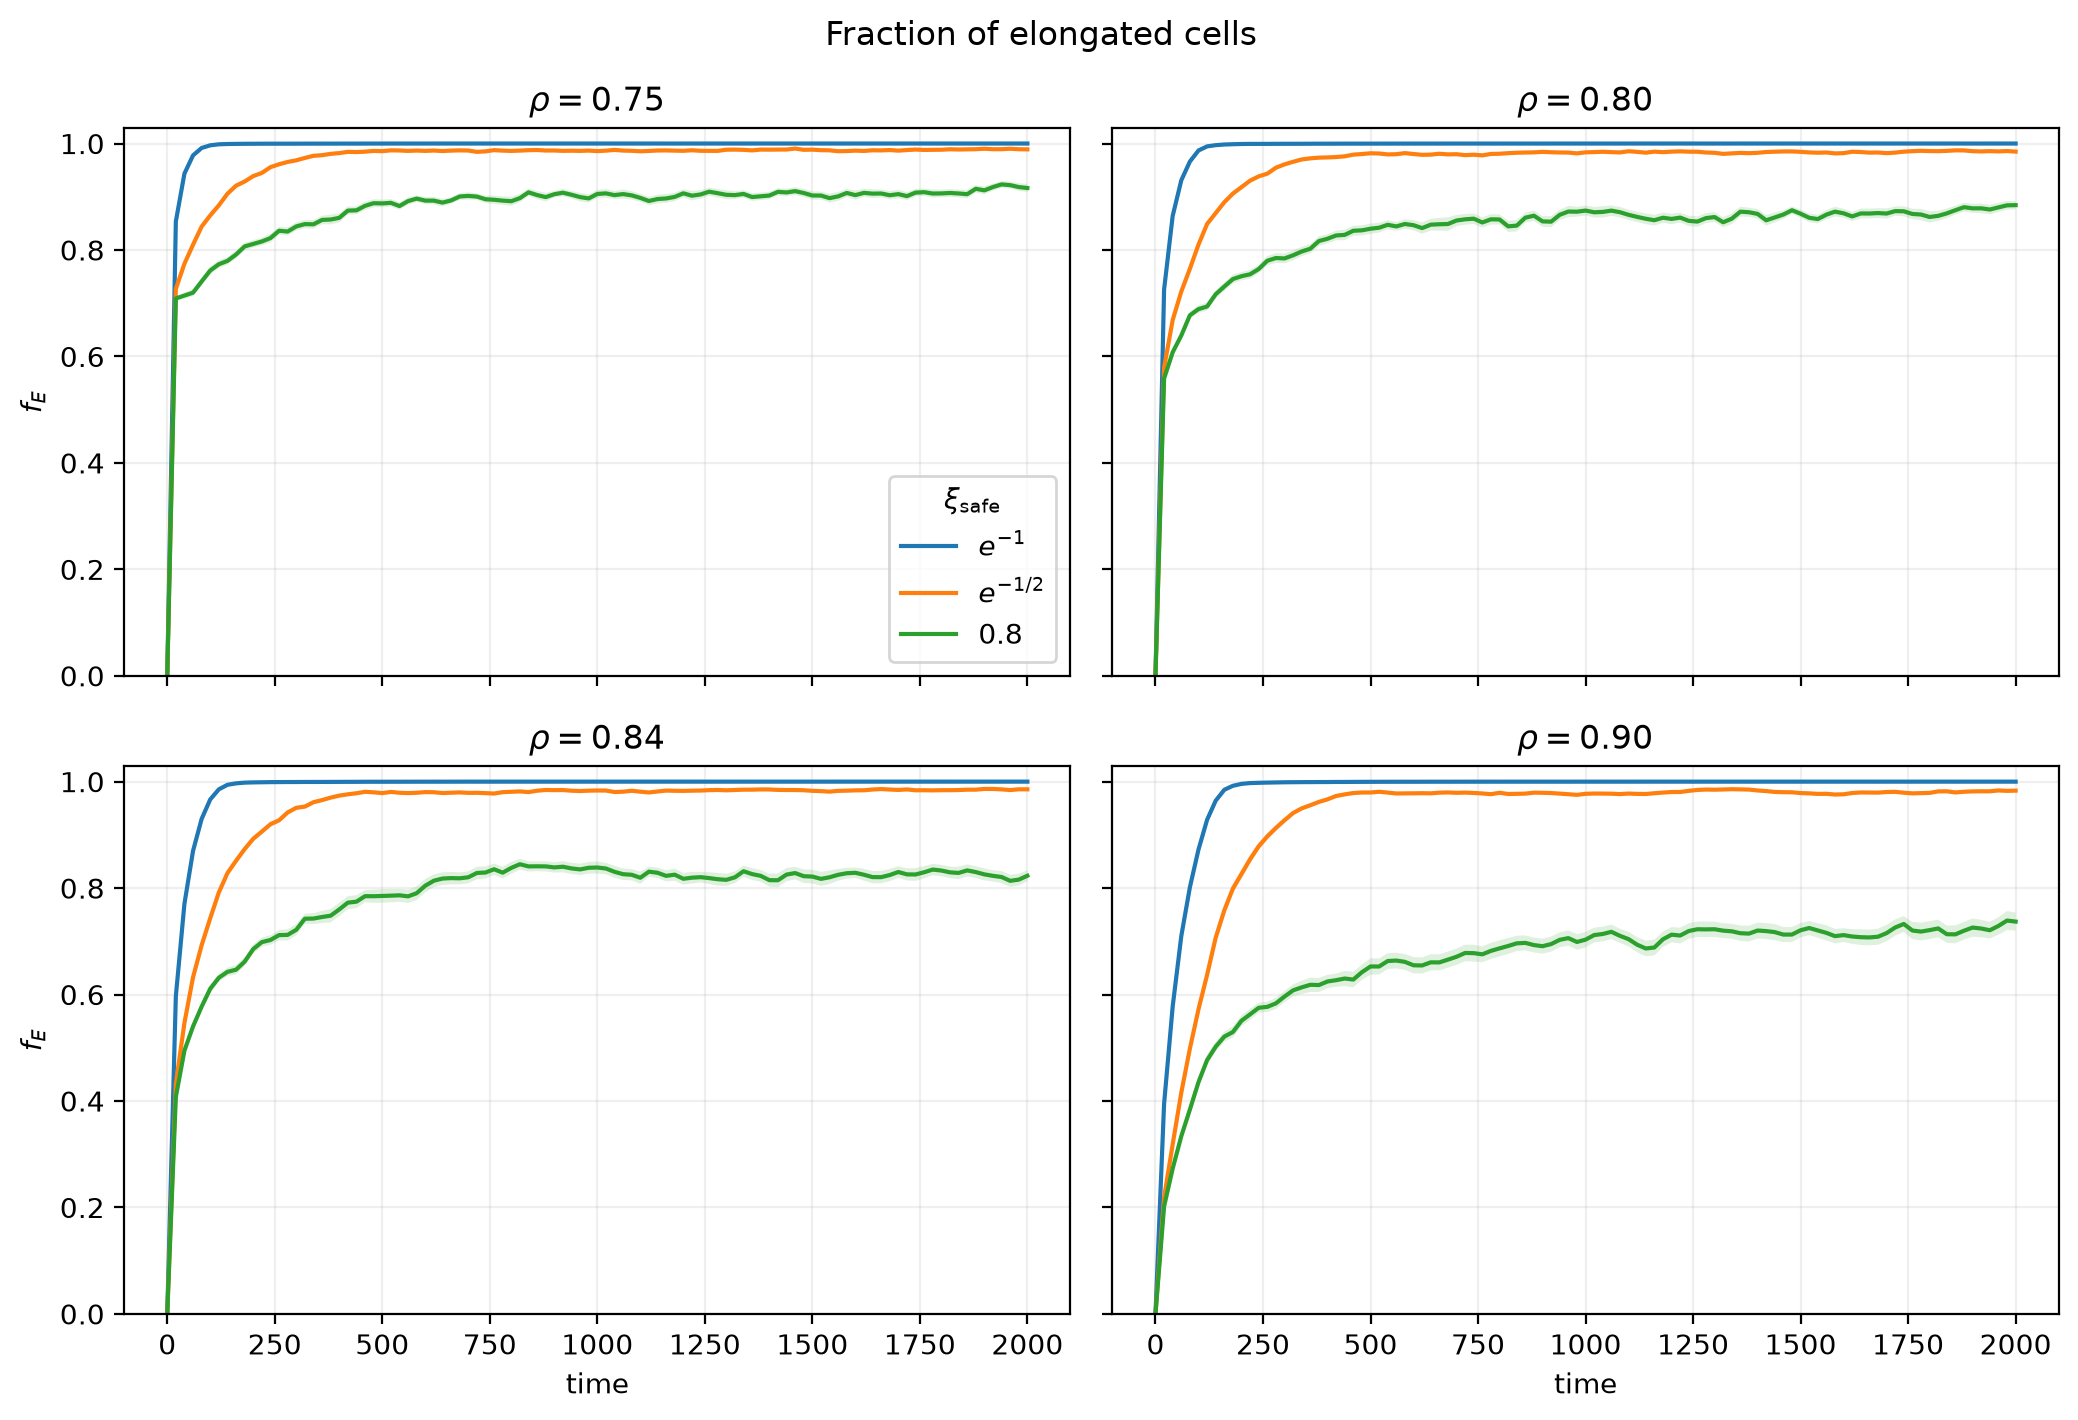
\includegraphics[width=0.92\textwidth]
    {../figures/fraction_elongated_time_series.png}
    \caption{
        Evolución temporal de la fracción de células elongadas para los tres
        umbrales de seguridad. Las líneas muestran la media de ensamble y las
        bandas el error estándar entre las 64 realizaciones.
    }
    \label{fig:fraction}
\end{figure}

\subsection{Intervención de la regla de seguridad}

La cantidad más directa para evaluar si el umbral controla la dinámica es la
fracción de contracciones rechazadas,

\begin{equation}
    r_{\rm reject}
    =
    \frac{N_{\rm rejected}}
         {N_{\rm accepted}+N_{\rm rejected}}.
\end{equation}

Los resultados muestran una separación muy marcada entre los tres valores.
Para $\xi_{\rm safe}=e^{-1}$ se rechaza aproximadamente
$99.98--99.99\%$ de las contracciones solicitadas mecánicamente.
Para $\xi_{\rm safe}=e^{-1/2}$ la fracción sigue siendo muy alta,
aproximadamente $92.2--95.9\%$.
En cambio, para $\xi_{\rm safe}=0.8$ sólo se rechaza
aproximadamente $0.84--1.15\%$.

La figura~\ref{fig:deformation} muestra además que, para
$\xi_{\rm safe}=0.8$, las tasas tardías de elongación y contracción permanecen
prácticamente balanceadas. Por lo tanto, la fracción elongada corresponde a un
balance dinámico entre ambos estados y no a una acumulación causada por la
regla de seguridad.

\begin{figure}[htbp]
    \centering
    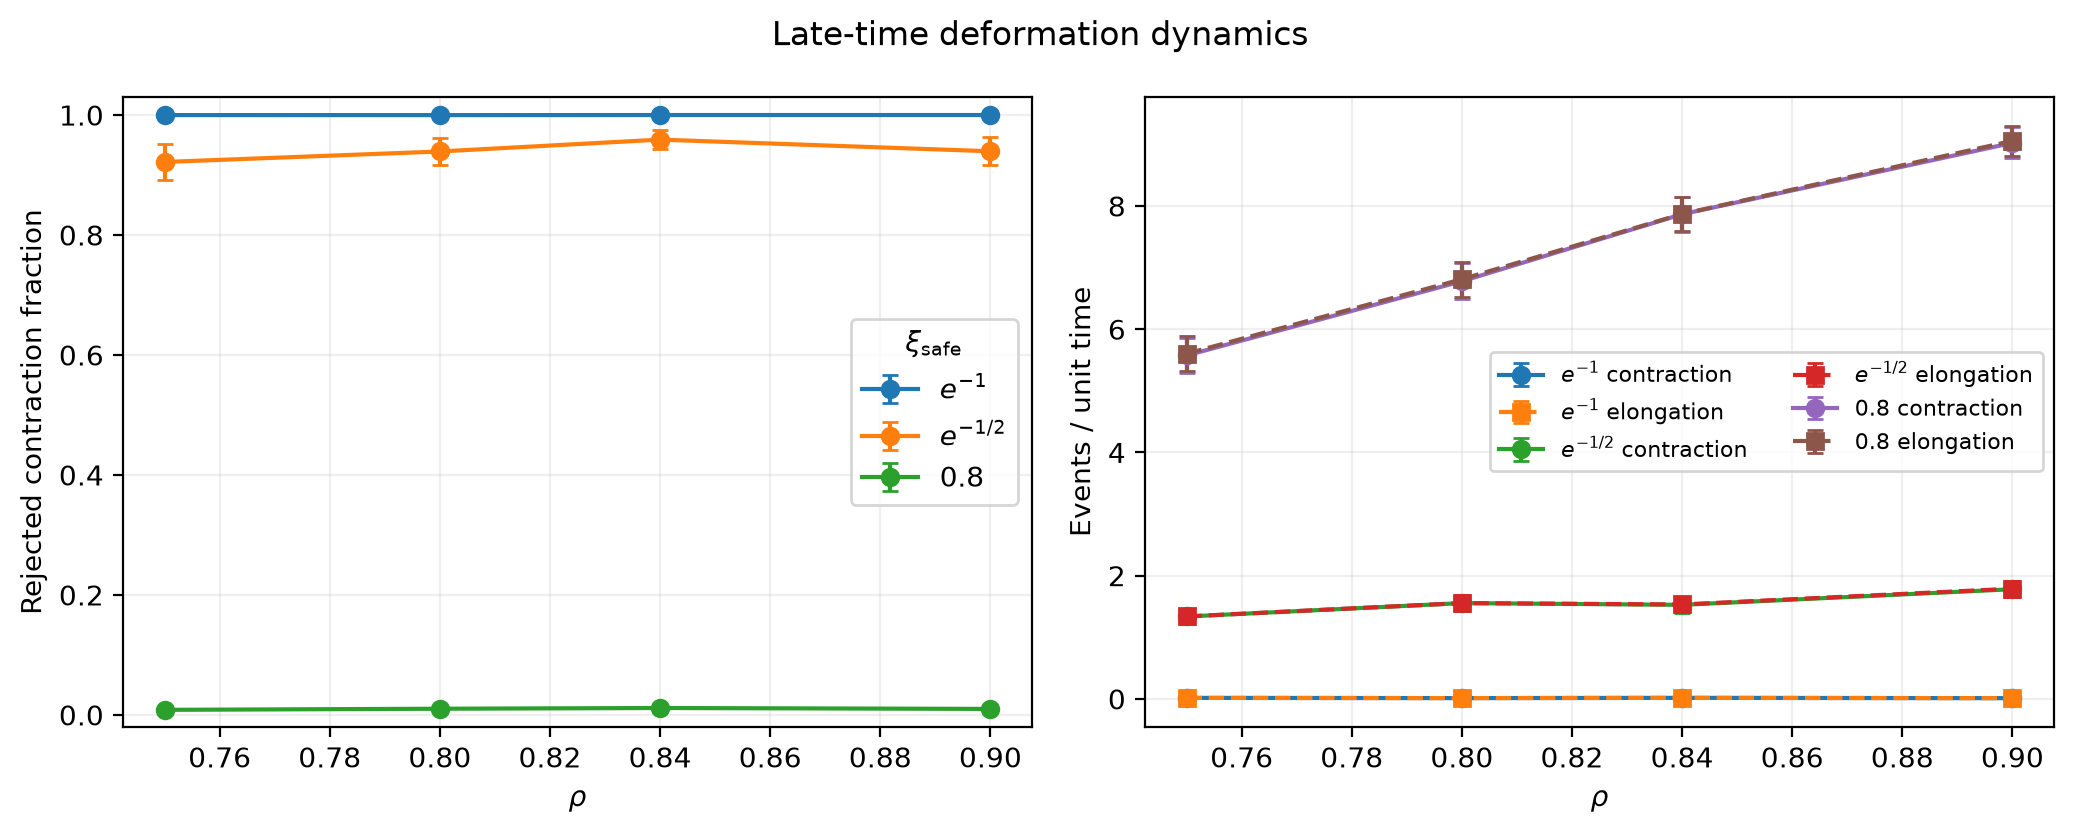
\includegraphics[width=0.92\textwidth]
    {../figures/deformation_dynamics_vs_xi_safe.png}
    \caption{
        Dinámica de deformación en la ventana tardía.
        Izquierda: fracción de contracciones rechazadas por la regla de
        seguridad. Derecha: tasas de elongaciones exitosas y contracciones
        aceptadas.
    }
    \label{fig:deformation}
\end{figure}

\subsection{Superposiciones}

Finalmente verificamos que el valor permisivo no elimine la función protectora
del umbral. La figura~\ref{fig:overlap} compara la cola de las
superposiciones propuestas y aceptadas después de una contracción con el
solapamiento medio del sistema.

Para $\xi_{\rm safe}=0.8$, las propuestas pueden superar ligeramente el
umbral, mientras que las contracciones aceptadas quedan limitadas por la regla.
Al mismo tiempo, el solapamiento normalizado medio permanece en un régimen
similar para los tres valores, aproximadamente entre $0.096$ y $0.107$ en las
densidades estudiadas. Esto indica que el umbral actúa principalmente sobre la
cola extrema asociada a las contracciones instantáneas, y no sobre el estado
típico de superposición del sistema.

\begin{figure}[htbp]
    \centering
    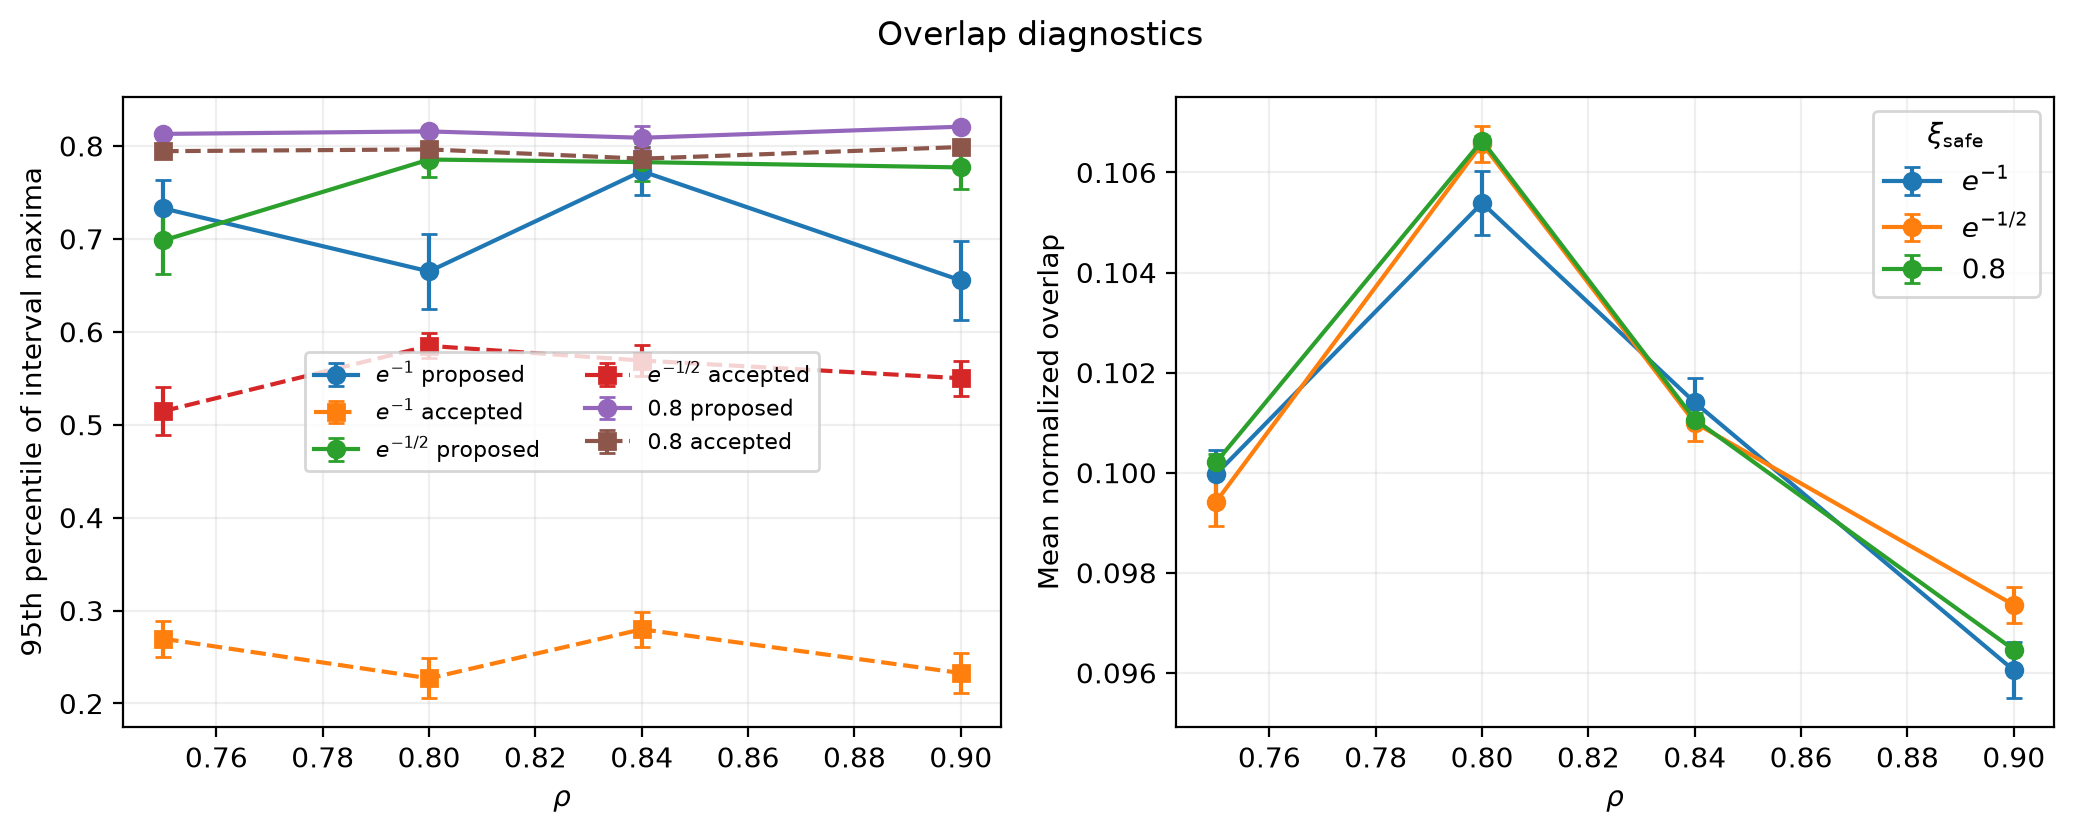
\includegraphics[width=0.92\textwidth]
    {../figures/overlap_diagnostics_vs_xi_safe.png}
    \caption{
        Diagnósticos de superposición en la ventana tardía.
        Izquierda: percentil 95 de la máxima superposición propuesta y aceptada
        en los intervalos de salida. Derecha: superposición normalizada media
        del sistema.
    }
    \label{fig:overlap}
\end{figure}

\section{Elección de \(\xi_{\rm safe}\)}

Los valores estrictos no se comportan como simples salvaguardas numéricas.
Al rechazar la gran mayoría de las contracciones, modifican directamente el
balance morfológico y llevan al sistema hacia un estado casi completamente
elongado.

Por el contrario, $\xi_{\rm safe}=0.8$ conserva la función de seguridad sobre
las contracciones de mayor superposición, pero interviene sólo en alrededor
del $1\%$ de los eventos solicitados. Por lo tanto, se adopta

\begin{equation}
    \boxed{\xi_{\rm safe}=0.8}.
\end{equation}

Con esta elección quedan fijados los principales elementos del protocolo
preliminar:

\begin{equation}
    \boxed{
        \lambda_{\rm core}=1,\qquad
        \Delta t=0.01,\qquad
        n_{\rm int}=5,\qquad
        \xi_{\rm safe}=0.8
    }.
\end{equation}

La morfología se actualiza una vez por paso de integración. El horizonte
temporal y la ventana tardía no se consideran parámetros universales del
modelo, sino cantidades que deberán verificarse en cada campaña física según
los tiempos de relajación correspondientes.

\end{document}
